\chapter{Describing a Chemical System: Extent, Activities, Q and K}\label{ch:b1:extent-q-and-k}

A hydrogen plant feeds natural gas and steam into tubes heated red-hot;
what comes out is never pure hydrogen but a mixture of hydrogen, carbon
monoxide, carbon dioxide, unreacted methane and steam, whose proportions
the engineers must know before they design the next unit. Predicting the
composition that leaves a reactor --- the final state of a chemical
system --- is the subject of this chapter. It needs a precise
description of the system (its variables and its composition), a single
number that measures how far a reaction has gone (the extent), and the
law that tells where the reaction stops (the equilibrium constant).
These tools are used in every later chapter on solutions.

\begin{recall}
Book 1 (grade 10) followed a reaction with a progress table and found the
\omterm{def:b1:extent-q-and-k:max-extent}{limiting reactant}; Book 1 (grade 12) introduced the \omterm{def:b1:extent-q-and-k:quotient}{reaction quotient}
$Q$ and the equilibrium constant $K$ of a non-total reaction. From
physics we use the perfect-gas law $pV = nRT$, with $R =
\qty{8.314}{J/(mol.K)}$.
\end{recall}

\begin{omfigure}
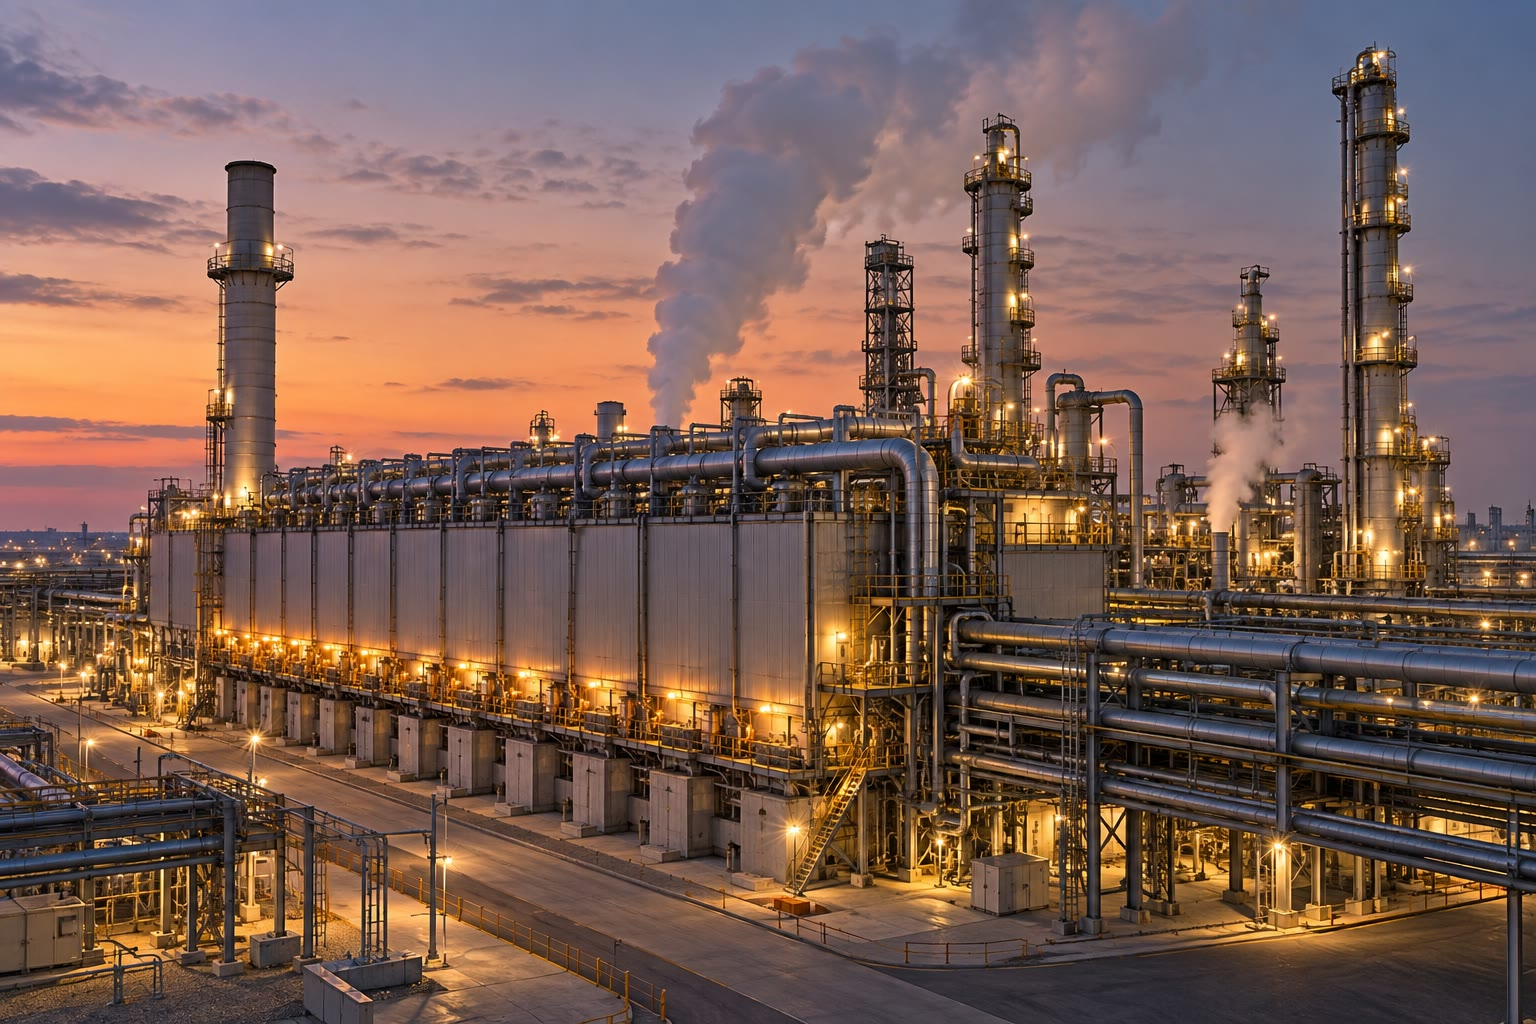
\includegraphics[width=0.6\linewidth]{images/book2/ai/b1-07-hydrogen-plant.jpg}

{\small A hydrogen plant at dusk. Natural gas and steam react in the
long reformer furnace; a second reactor converts carbon monoxide; the
outlet composition is a final state of the kind computed in this
chapter.}
\end{omfigure}

\section{Describing a system}

\begin{definition}[System, phase]\label{def:b1:extent-q-and-k:system}
A \emph{physico-chemical system}\index{physico-chemical system} is the
matter contained in a chosen region of space, the rest being its
surroundings. It is a \emph{closed system}\index{closed system} if it
exchanges no matter with the surroundings (it may exchange energy). A
\emph{phase}\index{phase} is a part of the system in which the \omterm{def:b1:extent-q-and-k:variables}{intensive
variables} vary continuously: a gas mixture is one phase, two immiscible
liquids are two phases, each solid is a phase of its own.
\end{definition}

\begin{definition}[Intensive and extensive variables]\label{def:b1:extent-q-and-k:variables}
A variable of state is \emph{extensive}\index{extensive variable} if it
is proportional to the size of the system (mass, volume, amount of
substance) and \emph{intensive}\index{intensive variable} if it is not
(temperature, pressure, concentration, density, \omterm{def:b1:extent-q-and-k:composition}{mole fraction}). The ratio
of two extensive variables is intensive.
\end{definition}

\begin{definition}[Composition variables]\label{def:b1:extent-q-and-k:composition}
For a constituent $i$ of a \omterm{def:b1:extent-q-and-k:system}{phase} containing the amounts $n_j$ of all its
constituents:
\begin{itemize}
  \item its \emph{mole fraction}\index{mole fraction} is $x_i = n_i/\sum_j
        n_j$, and its \emph{mass fraction}\index{mass fraction} $w_i =
        m_i/\sum_j m_j$; both lie between 0 and 1 and sum to 1;
  \item in a solution of volume $V$, its \emph{molar
        concentration}\index{molar concentration} is $c_i = [i] = n_i/V$,
        in \unit{mol/L};
  \item in a gas mixture at total pressure $p$, its \emph{partial
        pressure}\index{partial pressure} is $p_i = x_i\,p$.
\end{itemize}
\end{definition}

\begin{proposition}[Partial pressures of perfect gases]\label{prop:b1:extent-q-and-k:dalton}
In a mixture of perfect gases of volume $V$ at temperature $T$, the
\omterm{def:b1:extent-q-and-k:composition}{partial pressure} of a constituent is the pressure it would exert alone in
the whole volume, $p_i = n_iRT/V$, and the \omterm{def:b1:extent-q-and-k:composition}{partial pressures} add up to the
total pressure: $\sum_i p_i = p$.
\end{proposition}

\begin{proof}
For the mixture $pV = (\sum_j n_j)RT$, so $p_i = x_i p = \frac{n_i}{\sum_j
n_j}\cdot\frac{(\sum_j n_j)RT}{V} = \frac{n_iRT}{V}$, and $\sum_i x_i = 1$
gives $\sum_i p_i = p$.
\end{proof}

\begin{example}[Air]\label{ex:b1:extent-q-and-k:air}
Dry air contains, by volume (that is, by amount, for perfect gases),
78.08\,\% dinitrogen, 20.95\,\% dioxygen and 0.93\,\% argon. Under
\qty{1.013}{bar} the \omterm{def:b1:extent-q-and-k:composition}{partial pressure} of dioxygen is $0.2095 \times
1.013 = \qty{0.212}{bar}$; on a mountain where the pressure is
\qty{0.70}{bar}, it falls to \qty{0.147}{bar}, though the composition is
the same.
% ledger: air:N2, air:O2, air:Ar, const:atm
\end{example}

\section{Extent of reaction}

\begin{definition}[Stoichiometric numbers, extent]\label{def:b1:extent-q-and-k:extent}
A reaction is written $0 = \sum_i \nu_i\,\mathrm{A}_i$, where the
\emph{stoichiometric number}\index{stoichiometric number} $\nu_i$ of
species $\mathrm{A}_i$ is negative for a reactant and positive for a
product: in \ce{N2 + 3H2 -> 2NH3}, $\nu(\ce{N2}) = -1$, $\nu(\ce{H2}) = -3$,
$\nu(\ce{NH3}) = +2$. In a \omterm{def:b1:extent-q-and-k:system}{closed system} where this reaction alone takes
place, the amounts change as
\[
  n_i = n_{i,0} + \nu_i\,\xi ,
\]
which defines the \emph{extent of reaction}\index{extent of reaction}
$\xi$ (in moles), zero at the start and the same for every species.
\end{definition}

\begin{definition}[Maximum extent, limiting reactant]\label{def:b1:extent-q-and-k:max-extent}
The \emph{maximum extent}\index{maximum extent} $\xi_{\max}$ is the largest
value of $\xi$ for which no amount is negative: $\xi_{\max} = \min_{\nu_i <
0} n_{i,0}/|\nu_i|$. The reactant that reaches zero at $\xi_{\max}$ is the
\emph{limiting reactant}\index{limiting reactant}. When the extent can
also be negative (the reverse reaction), $\xi_{\min} = -\min_{\nu_i > 0}
n_{i,0}/\nu_i$.
\end{definition}

\begin{method}[The progress table]\label{met:b1:extent-q-and-k:progress-table}
To follow a reaction in a \omterm{def:b1:extent-q-and-k:system}{closed system}:
\begin{enumerate}
  \item write the balanced equation, and below it one column per species;
  \item first row: the initial amounts $n_{i,0}$;
  \item second row: the amounts at extent $\xi$, $n_{i,0} + \nu_i\xi$;
  \item for gases add a column with the total amount $n_{\text{tot}}(\xi)$;
  \item compute $\xi_{\max}$ (and $\xi_{\min}$) and identify the \omterm{def:b1:extent-q-and-k:max-extent}{limiting
        reactant};
  \item last row: the final amounts, at the final extent $\xi_f$ (found
        from the equilibrium condition, or equal to $\xi_{\max}$ if the
        reaction is total).
\end{enumerate}
\end{method}

\begin{example}[Synthesis of ammonia]\label{ex:b1:extent-q-and-k:ammonia}
From \qty{2.0}{mol} of \ce{N2} and \qty{3.0}{mol} of \ce{H2}:
\begin{center}
\begin{tabular}{lcccc}
\hline
 & \ce{N2} & \ce{3H2} & \ce{2NH3} & total \\
\hline
initial & 2.0 & 3.0 & 0 & 5.0 \\
extent $\xi$ & $2.0 - \xi$ & $3.0 - 3\xi$ & $2\xi$ & $5.0 - 2\xi$ \\
\hline
\end{tabular}
\end{center}
$\xi_{\max} = \min(2.0/1,\ 3.0/3) = \qty{1.0}{mol}$: dihydrogen is limiting.
If the reaction were total, the final state would hold \qty{1.0}{mol}
\ce{N2} and \qty{2.0}{mol} \ce{NH3}.
\end{example}

\begin{definition}[Final fractional extent, yield]\label{def:b1:extent-q-and-k:fractional-extent}
The \emph{final fractional extent}\index{final fractional extent} of a
reaction is $\tau = \xi_f/\xi_{\max}$, between 0 and 1. In a synthesis, the
\emph{yield}\index{yield} of a product is the ratio of the amount obtained
to the amount that the \omterm{def:b1:extent-q-and-k:max-extent}{limiting reactant} would give if the reaction were
total; when the product is not lost during isolation, it equals $\tau$.
\end{definition}

\section{Activities}

\begin{definition}[Standard state, activity]\label{def:b1:extent-q-and-k:activity}
The \emph{activity}\index{activity} $a_i$ of a species is a dimensionless
number that measures, in the expression of equilibrium laws, how much of
it is available; it is defined relative to a \emph{standard
state}\index{standard state}, a reference state at the temperature
considered and under the standard pressure $p^\circ = \qty{1}{bar}$. In
the ideal approximations used in this book:
\begin{itemize}
  \item for a gas, $a_i = p_i/p^\circ$ (the standard state is the pure
        perfect gas at $p^\circ$);
  \item for a solute in a dilute solution, $a_i = c_i/c^\circ$ with
        $c^\circ = \qty{1}{mol/L}$;
  \item for the solvent of a dilute solution, and for a pure solid or a
        pure liquid alone in its \omterm{def:b1:extent-q-and-k:system}{phase}, $a_i = 1$.
\end{itemize}
\end{definition}
% ledger: const:pstd

\begin{remark}[Ideal and real]\label{rem:b1:extent-q-and-k:ideal}
These expressions hold for perfect gases and for dilute solutions. In
concentrated solutions ions attract and repel one another and the
\omterm{def:b1:extent-q-and-k:activity}{activity} departs from $c_i/c^\circ$; the corrections, written with
\omterm{def:b1:extent-q-and-k:activity}{activity} coefficients, are studied in the Year 2 volume with the chemical
potential. For the concentrations used in this book (below about
\qty{0.1}{mol/L}) the ideal expressions are accurate to a few per cent.
\end{remark}

\section{The reaction quotient and the equilibrium constant}

\begin{definition}[Reaction quotient]\label{def:b1:extent-q-and-k:quotient}
The \emph{reaction quotient}\index{reaction quotient} of a reaction
$0 = \sum_i \nu_i\,\mathrm{A}_i$ in a given state of the system is
\[
  Q = \prod_i a_i^{\nu_i} ,
\]
the product of the activities of the products divided by that of the
reactants, each raised to the power of its stoichiometric coefficient.
\end{definition}

\begin{example}[Three quotients]\label{ex:b1:extent-q-and-k:quotients}
For \ce{N2(g) + 3H2(g) <=> 2NH3(g)}: $Q = \dfrac{(p_{\ce{NH3}}/p^\circ)^2}
{(p_{\ce{N2}}/p^\circ)(p_{\ce{H2}}/p^\circ)^3}$. For
\ce{CH3COOH(aq) + H2O(l) <=> CH3COO^-(aq) + H3O+(aq)}: $Q =
\dfrac{[\ce{CH3COO-}][\ce{H3O+}]}{[\ce{CH3COOH}]\,c^\circ}$, the solvent
having \omterm{def:b1:extent-q-and-k:activity}{activity} 1. For \ce{CaCO3(s) <=> CaO(s) + CO2(g)}: $Q =
p_{\ce{CO2}}/p^\circ$, the solids having \omterm{def:b1:extent-q-and-k:activity}{activity} 1.
\end{example}

\begin{definition}[Standard equilibrium constant]\label{def:b1:extent-q-and-k:equilibrium-constant}
The \emph{standard equilibrium constant}\index{standard equilibrium constant}
$K^\circ$ of a reaction is the value taken by its \omterm{def:b1:extent-q-and-k:quotient}{reaction
quotient} when the system is at equilibrium. It is dimensionless and
depends only on the reaction and the temperature.
\end{definition}

\begin{theorem}[Law of mass action]\label{thm:b1:extent-q-and-k:mass-action}
At a given temperature, a system in which a reaction can take place in
both directions evolves until $Q = K^\circ(T)$; at equilibrium, whatever
the initial composition,
\[
  \prod_i a_{i,\text{eq}}^{\nu_i} = K^\circ(T) .
\]
\end{theorem}
\admitted

\begin{proposition}[Direction of evolution]\label{prop:b1:extent-q-and-k:direction}
A system in which $Q < K^\circ$ evolves in the forward direction ($\xi$
increases); if $Q > K^\circ$, it evolves in the reverse direction; if
$Q = K^\circ$, it is at equilibrium.
\end{proposition}
\admitted

\begin{remark}[Where these laws come from]\label{rem:b1:extent-q-and-k:origin}
Both statements follow from the second law of thermodynamics, through the
free energy of reaction and the chemical potentials of the species: they
are derived in the Year 2 volume, which also gives $K^\circ$ from tables
of thermodynamic data and explains how it changes with temperature. Here
they are used as laws.
\end{remark}

\begin{omfigure}
\begin{tikzpicture}[font=\small, >={Stealth}]
  \draw[->, thick] (0,0) -- (11,0) node[right] {$Q$};
  \draw[thick, omThm] (5.5,0.25) -- (5.5,-0.25) node[below] {$K^\circ$};
  \draw[->, omDef, thick] (1.0,0.55) -- (4.6,0.55);
  \node[above, omDef] at (2.8,0.6) {$Q < K^\circ$: forward};
  \draw[->, omProp, thick] (10.0,0.55) -- (6.4,0.55);
  \node[above, omProp] at (8.2,0.6) {$Q > K^\circ$: reverse};
  \node[below] at (0,-0.1) {0};
\end{tikzpicture}

{\small The quotient moves towards the constant: a system with $Q <
K^\circ$ makes products, one with $Q > K^\circ$ consumes them.}
\end{omfigure}

\begin{proposition}[Combining constants]\label{prop:b1:extent-q-and-k:combine-k}
If $K_1^\circ$ and $K_2^\circ$ are the constants of reactions (1) and (2):
the reverse of (1) has the constant $1/K_1^\circ$; the reaction $n \times
(1)$ has $(K_1^\circ)^n$; the sum $(1) + (2)$ has $K_1^\circ K_2^\circ$.
\end{proposition}

\begin{proof}
The quotient of the reverse reaction is $\prod a_i^{-\nu_i} = 1/Q_1$; that
of $n \times (1)$ is $\prod a_i^{n\nu_i} = Q_1^n$; that of the sum is
$\prod a_i^{\nu_{i,1} + \nu_{i,2}} = Q_1 Q_2$. Writing these identities at
equilibrium, where each quotient equals its constant, gives the result.
\end{proof}

\begin{proposition}[One equilibrium state]\label{prop:b1:extent-q-and-k:q-monotone}
For a single reaction in a \omterm{def:b1:extent-q-and-k:system}{closed system} at fixed temperature (and, for
gases, fixed volume or pressure), the quotient $Q(\xi)$ is a strictly
increasing function of $\xi$ on $(\xi_{\min}, \xi_{\max})$, going from 0
to $+\infty$ when no species of constant \omterm{def:b1:extent-q-and-k:activity}{activity} is involved. The
equation $Q(\xi) = K^\circ$ then has exactly one solution in this
interval.
\end{proposition}

\begin{proof}
Take a solution reaction, $Q(\xi) = \prod_i (n_{i,0} + \nu_i\xi)^{\nu_i}
\times \text{const}$. Its logarithmic derivative is
\[
  \frac{\dd \ln Q}{\dd \xi} = \sum_i \frac{\nu_i^2}{n_{i,0} + \nu_i \xi}
  > 0 ,
\]
each term being positive where all amounts are. As $\xi \to \xi_{\max}$ a
reactant amount tends to 0 in a denominator and $Q \to +\infty$; as $\xi
\to \xi_{\min}$ a product amount tends to 0 and $Q \to 0$. A continuous
increasing function from 0 to $+\infty$ takes the value $K^\circ$ once.
(For gases at constant pressure, the total amount also varies; the result
still holds, as can be checked in each case.)
\end{proof}

\section{Final states}

\begin{definition}[Equilibrium state, quantitative reaction]\label{def:b1:extent-q-and-k:quantitative}
The final state is an \emph{equilibrium state}\index{equilibrium state}
when all the species of the reaction are present and $Q = K^\circ$. The
reaction is \emph{quantitative}\index{quantitative reaction} (or total)
when at the final state the \omterm{def:b1:extent-q-and-k:max-extent}{limiting reactant} has practically
disappeared, $\xi_f \approx \xi_{\max}$; this happens when $K^\circ$ is
very large.
\end{definition}

\begin{method}[Finding the final state]\label{met:b1:extent-q-and-k:final-state}
To find the final state of a single reaction:
\begin{enumerate}
  \item draw the progress table and compute $\xi_{\max}$ (and $\xi_{\min}$);
  \item compute $Q$ at the start and compare it with $K^\circ$ to find the
        direction;
  \item express $Q(\xi)$ with the activities and solve $Q(\xi) = K^\circ$
        for $\xi$ in $(\xi_{\min}, \xi_{\max})$;
  \item if a species of \omterm{def:b1:extent-q-and-k:activity}{activity} 1 (a solid) is involved, check that it is
        still present at that extent: if it would have to become negative,
        it disappears first and the final state is \emph{not} an
        equilibrium ($\xi_f = \xi_{\max}$, $Q_f \ne K^\circ$).
\end{enumerate}
\end{method}

\begin{method}[The quantitative-reaction hypothesis]\label{met:b1:extent-q-and-k:quantitative}
When $K^\circ$ is large (typically above $10^4$), assume the reaction
total: set $\xi_f = \xi_{\max}$, compute the final amounts, then find the
small amount $\varepsilon$ of the \omterm{def:b1:extent-q-and-k:max-extent}{limiting reactant} left by writing $Q =
K^\circ$ with the other amounts unchanged. The hypothesis is accepted if
$\varepsilon$ is small compared with the other amounts (below about
1\,\%).
\end{method}

\begin{example}[A quantitative reaction]\label{ex:b1:extent-q-and-k:quant}
For $\mathrm{A + B \rightleftharpoons C + D}$ in solution with $[\ce{A}]_0 = [\ce{B}]_0 =
\qty{0.10}{mol/L}$ and $K^\circ = 10^6$: assuming total reaction, $[\ce{C}]
= [\ce{D}] = 0.10$; then $0.10^2/\varepsilon^2 = 10^6$ gives $\varepsilon
= \qty{1.0e-4}{mol/L}$, 0.1\,\% of the initial amount: the hypothesis is
justified.
\end{example}

\begin{omfigure}
\begin{tikzpicture}
\begin{axis}[
  width=0.45\linewidth, height=5.6cm, ymode=log,
  xmin=0, xmax=1, ymin=0.01, ymax=1000,
  axis x line=bottom, axis y line=left,
  xlabel={extent $\xi$ (mol)}, ylabel={$Q$}, xtick={0,0.2,0.4,0.8,1},
  tick label style={font=\small}, label style={font=\small}, clip=false]
\addplot[omDef, thick] table[x=xi, y=Q] {figdata/out/bachelor-1-extent-equilibrium-shift.dat};
\draw[omThm, dashed] (axis cs:0,4) -- (axis cs:1,4);
\node[omThm, anchor=south west, font=\small] at (axis cs:0.02,4) {$K^\circ = 4.0$};
\draw[dotted] (axis cs:0.607,0.01) -- (axis cs:0.607,4);
\node[anchor=north, font=\small] at (axis cs:0.607,0.01) {0.607};
\end{axis}
\end{tikzpicture}\hfill
\begin{tikzpicture}
\begin{axis}[
  width=0.45\linewidth, height=5.6cm,
  xmin=0, xmax=0.04, ymin=0, ymax=0.3,
  axis x line=bottom, axis y line=left,
  xlabel={extent $\xi$ (mol)}, ylabel={$Q = p_{\ce{CO2}}/p^\circ$},
  xtick={0,0.01,0.02,0.03,0.04}, scaled x ticks=false,
  xticklabel style={/pgf/number format/fixed, /pgf/number format/precision=2},
  yticklabel style={/pgf/number format/fixed},
  tick label style={font=\small}, label style={font=\small}, clip=false]
\addplot[omProp, thick] table[x=xi, y=Q_small] {figdata/out/bachelor-1-extent-equilibrium-carbonate.dat};
\addplot[omDef, thick, dashed] table[x=xi, y=Q_large] {figdata/out/bachelor-1-extent-equilibrium-carbonate.dat};
\draw[omThm, dashed] (axis cs:0,0.2) -- (axis cs:0.04,0.2);
\node[omThm, anchor=south west, font=\small] at (axis cs:0.0005,0.2) {$K^\circ = 0.20$};
\node[omProp, anchor=north west, font=\scriptsize] at (axis cs:0.012,0.088) {\qty{0.010}{mol}: solid gone};
\node[omDef, anchor=north west, font=\scriptsize] at (axis cs:0.024,0.19) {\qty{0.050}{mol}: equilibrium};
\end{axis}
\end{tikzpicture}

{\small Left: the quotient of \ce{CO + H2O <=> CO2 + H2} rises with the
extent and meets $K^\circ$ once (weekend problem). Right: for
\ce{CaCO3(s) <=> CaO(s) + CO2(g)} in a closed \qty{10}{L} vessel,
$Q = p_{\ce{CO2}}/p^\circ$ grows with $\xi$; with \qty{0.050}{mol} of
carbonate it reaches $K^\circ = 0.20$ (equilibrium), with \qty{0.010}{mol}
the carbonate is exhausted first and the final state is not an
equilibrium.}
\end{omfigure}

\begin{method}[Two simultaneous reactions]\label{met:b1:extent-q-and-k:two-reactions}
When two reactions take place in the same system, give each its own
extent, $\xi_1$ and $\xi_2$; every amount is $n_i = n_{i,0} + \nu_{i,1}\xi_1
+ \nu_{i,2}\xi_2$, and the final state satisfies both $Q_1 = K_1^\circ$ and
$Q_2 = K_2^\circ$ (a system of two equations). If one constant is much
larger than the other, treat the corresponding reaction first as
\omterm{def:b1:extent-q-and-k:quantitative}{quantitative}, then the second on the result.
\end{method}

\begin{history}[The law of mass action, 1864]
In 1864 the Norwegian chemist Cato Guldberg and his brother-in-law, the
pharmacist Peter Waage, published in Norwegian their law of ``active
masses'': a reaction proceeds until the forces of the forward and reverse
reactions balance, each proportional to the concentrations of its
reactants. Their work went unnoticed abroad until they republished it in two more
widely read languages, in 1867 and 1879; Jacobus van 't Hoff, who had
rediscovered the law, acknowledged their priority.
\end{history}

\section{Exercises}

\begin{exercise}[$\star$]\label{exo:b1:extent-q-and-k:1}
Classify as \omterm{def:b1:extent-q-and-k:variables}{intensive} or \omterm{def:b1:extent-q-and-k:variables}{extensive}: temperature, volume, amount of
substance, \omterm{def:b1:extent-q-and-k:composition}{molar concentration}, density, pressure, mass, \omterm{def:b1:extent-q-and-k:composition}{mole fraction}.
\end{exercise}

\begin{exercise}[$\star$]\label{exo:b1:extent-q-and-k:2}
Using the composition of dry air given in the chapter, compute the
\omterm{def:b1:extent-q-and-k:composition}{partial pressures} of \ce{N2}, \ce{O2} and \ce{Ar} under a total pressure
of \qty{1.013}{bar}.
\end{exercise}

\begin{exercise}[$\star$]\label{exo:b1:extent-q-and-k:3}
Draw the progress table of \ce{2H2 + O2 -> 2H2O} from \qty{3.0}{mol} of
\ce{H2} and \qty{2.0}{mol} of \ce{O2}. Find $\xi_{\max}$, the \omterm{def:b1:extent-q-and-k:max-extent}{limiting
reactant} and the final state if the reaction is total.
\end{exercise}

\begin{exercise}[$\star$]\label{exo:b1:extent-q-and-k:4}
Write the \omterm{def:b1:extent-q-and-k:quotient}{reaction quotient} of: (a) \ce{CaCO3(s) <=> CaO(s) + CO2(g)};
(b) \ce{Ag+(aq) + Cl-(aq) <=> AgCl(s)}; (c) \ce{N2(g) + 3H2(g) <=>
2NH3(g)}; (d) \ce{NH3(aq) + H2O(l) <=> NH4+(aq) + OH-(aq)}.
\end{exercise}

\begin{exercise}[$\star\star$]\label{exo:b1:extent-q-and-k:5}
Reactions (1) $\mathrm{A \rightleftharpoons B}$ and (2) $\mathrm{B \rightleftharpoons C}$ have the constants
$K_1^\circ = 10$ and $K_2^\circ = 0.5$. Give the constants of $\mathrm{A \rightleftharpoons C}$,
$\mathrm{C \rightleftharpoons A}$ and $\mathrm{2\,A \rightleftharpoons 2\,C}$.
\end{exercise}

\begin{exercise}[$\star\star$]\label{exo:b1:extent-q-and-k:6}
A reaction has $K^\circ = 2.0 \times 10^{-3}$. In which direction does
the system evolve if, initially, $Q = 5.0 \times 10^{-5}$? If $Q = 0.10$?
If only reactants are present?
\end{exercise}

\begin{exercise}[$\star\star$]\label{exo:b1:extent-q-and-k:7}
The gas \ce{A2} dissociates, \ce{A2(g) <=> 2A(g)}, with $K^\circ = 0.25$ at
the temperature of the experiment. Starting from \qty{1.0}{mol} of \ce{A2}
under a total pressure kept at $p^\circ$, write the progress table with
the total amount, express $Q(\xi)$ and find the equilibrium extent.
\end{exercise}

\begin{exercise}[$\star\star$]\label{exo:b1:extent-q-and-k:8}
In solution, $\mathrm{A + B \rightleftharpoons C}$ with $K^\circ = 100$ and initial
concentrations $[\ce{A}]_0 = [\ce{B}]_0 = \qty{0.10}{mol/L}$. Find the
equilibrium concentrations and the \omterm{def:b1:extent-q-and-k:fractional-extent}{final fractional extent}.
\end{exercise}

\begin{exercise}[$\star\star$]\label{exo:b1:extent-q-and-k:9}
For $\mathrm{A + B \rightleftharpoons C + D}$ from equal amounts of \ce{A} and \ce{B}, show that
the \omterm{def:b1:extent-q-and-k:fractional-extent}{final fractional extent} is $\tau = \sqrt{K^\circ}/(1 + \sqrt{K^\circ})$.
What value of $K^\circ$ gives $\tau = 0.99$?
\end{exercise}

\begin{exercise}[$\star\star\star$]\label{exo:b1:extent-q-and-k:10}
Calcium carbonate is heated at \qty{1100}{K} in a closed vessel of
\qty{10.0}{L}, initially empty of gas, for which $K^\circ = 0.20$ for
\ce{CaCO3(s) <=> CaO(s) + CO2(g)}. Find the final state for
\qty{0.010}{mol} and for \qty{0.050}{mol} of carbonate.
\end{exercise}

\begin{exercise}[$\star\star\star$]\label{exo:b1:extent-q-and-k:11}
A substance \ce{A} isomerises in solution in two ways, $\mathrm{A \rightleftharpoons B}$
($K_1^\circ = 2.0$) and $\mathrm{A \rightleftharpoons C}$ ($K_2^\circ = 3.0$). Starting from
\qty{1.0}{mol} of \ce{A} alone, find the final amounts of the three
isomers.
\end{exercise}

\begin{exercise}[$\star\star\star$]\label{exo:b1:extent-q-and-k:12}
An acid \ce{A} and an alcohol \ce{B} give an ester and water, $\mathrm{A + B
\rightleftharpoons E + W}$, all in one liquid \omterm{def:b1:extent-q-and-k:system}{phase}, with $K^\circ = 4.0$ (take the
activities as the \omterm{def:b1:extent-q-and-k:composition}{mole fractions}; the total amount does not change).
Compute the maximum \omterm{def:b1:extent-q-and-k:fractional-extent}{yield} of ester from \qty{0.50}{mol} of each reactant,
then from \qty{0.50}{mol} of acid and \qty{1.0}{mol} of alcohol.
\end{exercise}

\section{Problem: The Outlet of a Hydrogen Plant}

\begin{problem}[{Weekend problem --- composition variables of a feed,
steam reforming treated as total, the water--gas shift at equilibrium,
and the hydrogen content of the gas leaving the plant}]
\label{pb:b1:extent-q-and-k:1}
A hydrogen plant is fed with \qty{1.00}{mol} of methane and
\qty{3.00}{mol} of steam (per unit of time) under \qty{30}{bar}. In the
reformer, \ce{CH4 + H2O -> CO + 3H2} is assumed total. In the shift
reactor, \ce{CO + H2O <=> CO2 + H2} reaches equilibrium; take $K^\circ =
4.0$ at its temperature. Molar masses: \ce{CH4} \qty{16.04}{g/mol},
\ce{H2O} \qty{18.02}{g/mol}.

\medskip
\noindent\textbf{Part I --- The feed.}
\begin{enumerate}
  \item Compute the \omterm{def:b1:extent-q-and-k:composition}{mole fractions} of methane and steam in the feed.
  \item Compute their \omterm{def:b1:extent-q-and-k:composition}{partial pressures}.
  \item Compute their \omterm{def:b1:extent-q-and-k:composition}{mass fractions}.
  \item Which of the quantities used so far are \omterm{def:b1:extent-q-and-k:variables}{intensive}?
  \item Give the activities of methane and steam in the feed.
\end{enumerate}

\medskip
\noindent\textbf{Part II --- Reforming.}
\begin{enumerate}[resume]
  \item Draw the progress table of the reforming reaction.
  \item Compute $\xi_{\max}$ and name the \omterm{def:b1:extent-q-and-k:max-extent}{limiting reactant}.
  \item Give the amounts leaving the reformer.
  \item Compute the total amount of gas, and compare it with the feed.
  \item Compute the \omterm{def:b1:extent-q-and-k:composition}{mole fractions} leaving the reformer.
  \item Why is steam fed in excess?
\end{enumerate}

\medskip
\noindent\textbf{Part III --- The shift reactor.}
\begin{enumerate}[resume]
  \item Draw the progress table of the shift reaction, starting from the
        gas leaving the reformer.
  \item Show that $Q(\xi) = \dfrac{\xi(3 + \xi)}{(1 - \xi)(2 - \xi)}$, and
        that it does not depend on the pressure.
  \item Compute $Q$ at the inlet and predict the direction of evolution.
  \item Write the equation for the equilibrium extent and solve it,
        keeping the root that makes sense.
  \item Give the amounts leaving the shift reactor.
  \item Compute the \omterm{def:b1:extent-q-and-k:fractional-extent}{final fractional extent} of the shift reaction.
  \item With twice as much steam in the feed (\qty{6.00}{mol}), the gas
        enters the shift reactor with \qty{5.00}{mol} of steam: compute the
        new equilibrium extent.
\end{enumerate}

\medskip
\noindent\textbf{Part IV --- What leaves the plant.}
\begin{enumerate}[resume]
  \item What value of $K^\circ$ would be needed to convert 99\,\% of the
        carbon monoxide in the first case?
  \item Explain why a shift reactor converts more when it runs at a
        temperature where its constant is larger, and why plants use two
        shift reactors in series.
  \item The steam is condensed out of the gas leaving the shift reactor.
        Compute the \omterm{def:b1:extent-q-and-k:composition}{mole fraction} of hydrogen in the dry gas.
  \item List the impurities that remain and their amounts.
  \item Compute the \omterm{def:b1:extent-q-and-k:composition}{mole fraction} of hydrogen in the gas leaving the shift
        reactor, steam included.
\end{enumerate}
\end{problem}
